\chapter{The Application Programming Interface}
\label{API}
	\section{Introduction}
		In this section, we will briefly discuss the communication protocol used by the application to its internal components. 
		As mentioned already in the previous chapters, the protocol used is a designed to be a stateful[\cite{session-rfc6265}], 
		JSON-based[\cite{json-rfc7159}], Https[\cite{rfc2818}], restful [\cite{restful-rfc7231}]protocol. Let us explain briefly 
		what those technical terms mean.
		\subsection{Stateful Protocol}
			
			
			A stateful protocol[\cite{session-rfc6265}] is a protocol capable of recognizing and distinguishing between the different requests made by the 
			same host machine.  In our application, this is essential because the authentication functionality would be impossible 
			otherwise. An authenticated user is always associated with a session. The session id[\cite{sessionID-rfc7329}] is a character string that is returned 
			after the authentication is complete and should be attached to every subsequent request for user authentication to work. 
			Our application protocol uses the cookie mechanism to attach the sessionID to every request, ensuring that the Services 
			will recognize the sender. The following image provides an example.
			\begin{figure}[H]
				\iftrue
				\caption{Session ID Attached to Notifications Request, captured using Firefox-Tools}
				\centering
				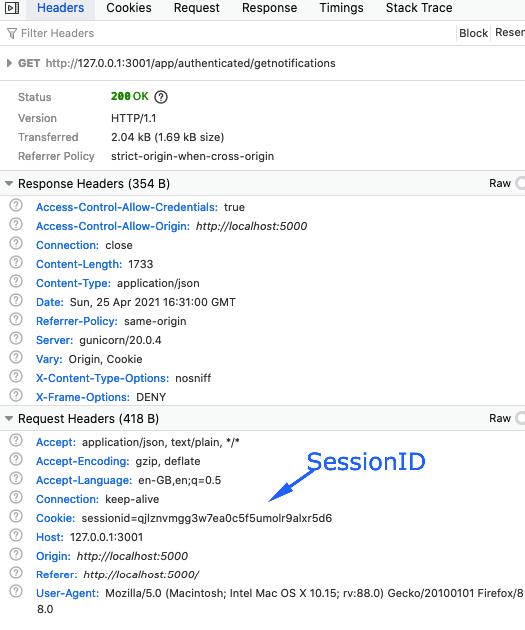
\includegraphics[scale=0.3]{figures/sessionID}
				\fi
			\end{figure} 
			Here, the Session ID is attached to a request from the Frontend Application into the Information Service for the retrieval of new notifications.
		\subsection{Json}
		
			The JavaScript Object Notation (or JSON) Data Interchange Format[\cite{json-rfc7159}] is a text-based, lightweight, human-readable language-independent 
			data exchange format. We use JSON extensively to design our communication protocol, mainly because of its widely adopted use and availability 
			of decoders. Additionally, both languages involved in the data transaction(javascript for the frontend, python for the backend services) 
			support JSON natively.
			\begin{figure}[H]
				\iftrue
				\caption{Capturing the Information service's JSON-Based responce using Postman}
				\centering
				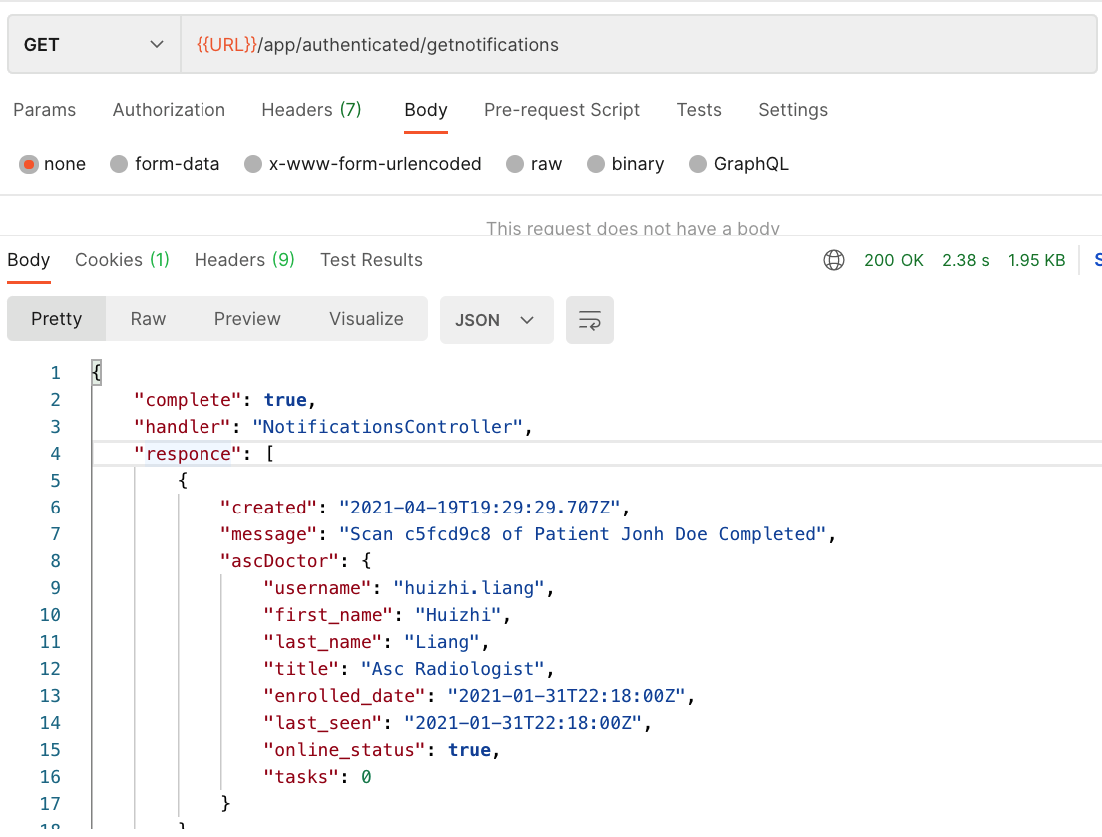
\includegraphics[scale=0.3]{figures/json}
				\fi
			\end{figure} 
		\subsection{HTTPS}
		
		
			HTTPS[\cite{rfc2818}] or HyperText Transfer Protocol Secure version is an updated version of the classic HTTP protocol, using TLS as an additional security layer. 
			TLS  encrypts all the underlying data to provide unparallel protection against various malicious attacks. The following images showed the login 
			packages as they were sent from the Frontend Application to the Information Service using the WireShark packet analyzer.

			\begin{figure}[H]
				\iftrue
				\caption{Unecrupted Credentials (HTTPS disabled)}
				\centering
				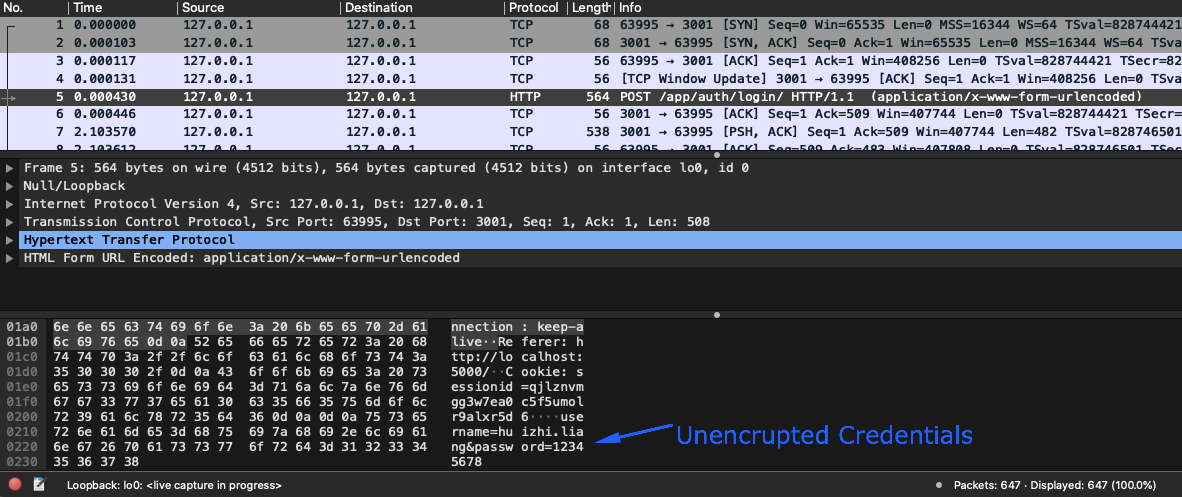
\includegraphics[scale=0.3]{figures/http}
				\fi
			\end{figure}
			\begin{figure}[H]
				\iftrue
				\caption{Ecrupted Credentials (HTTPS enabled)}
				\centering
				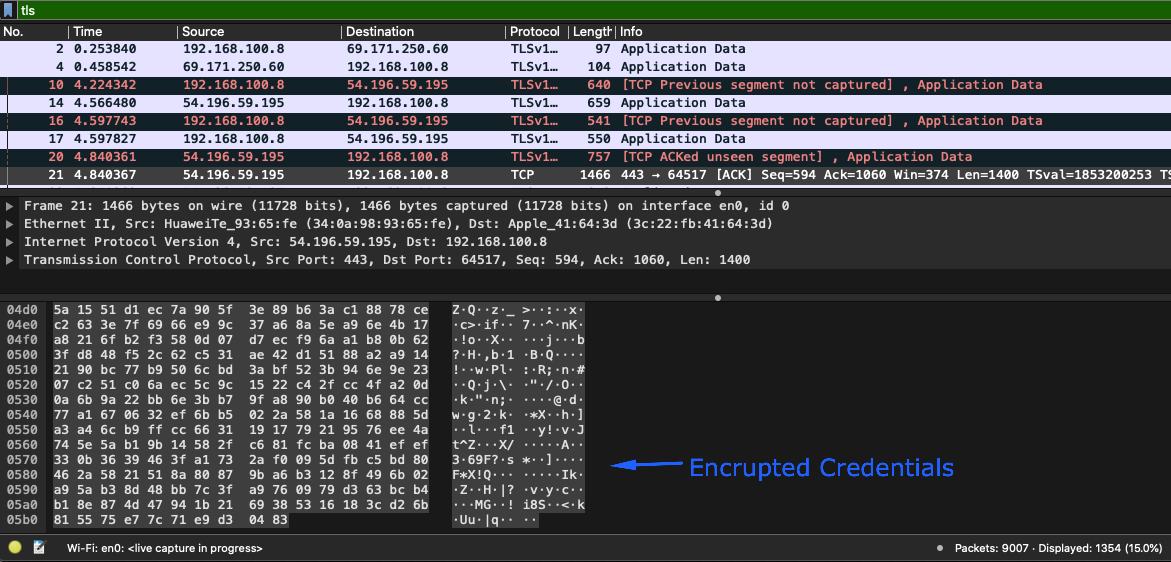
\includegraphics[scale=0.3]{figures/https}
				\fi
			\end{figure}
			It becomes evident that, by using HTTPS, we increase our system security, as credentials and personal information are encrypted before sent over the internet.
		\subsection{RESTFull protocol}
			A protocol is REpresentational State Transfer (REST) \cite{pautasso_zimmermann_leymann_2008}Full when its design enables the following criteria to be fullfiled.
			\subsubsection{Resource identification through URI.}
				A protocol is RESTFul if it exposes several resources which identify the targets of the interaction with its clients. 
				An example of this may be a contacts repository. The resources(contact repository) are identified via URIs[\cite{uri-rfc3986}].
			\subsection{Uniform Interface}
				A protocol is restFul if the exposed resources are manipulated through a fixed set of four operations. Those operations 
				have been encoded to the HTTP/HTTPS protocols themselves, making the creation of RESTFul APIs easier. The operations are
				\begin{itemize}
					\item PUT
					\item GET
					\item POST
					\item DELETE
				\end{itemize}
			\subsection{Self-descriptive messages}
				A protocol is RestFul if the underlying resource is decoupled of its representation, making the access of the resource possible 
				using a variety of different formats, such as JSON, XML, plain text, PDF, and others.
			\subsection{Stateful interactions through hyperlinks}
				A protocol is Restful if every interaction between the server and a client is stateless i.e., the request messages 
				are self-contained; hence any stateful interaction should be explicit and based on the contents of the message itself.
		\section{Protocol Specification}
			From now onwards, we will define and explain the various calls and responses that define our application protocol. This section 
			may be referenced by future development as complete documentation.
			\subsection{Definitions}
				Before we proceed with the complete specification, we need to define some technical terms.
				\subsubsection{Session}
					\label{session}
					
					A session[\cite{session-rfc6265}] is a mechanism utilized by all the stateful protocols relying on a stateless protocol for application transmission. 
					HTTP/HTTPS is the primary protocol for web communication, and our protocol relies on HTTP/HTTPS for data transmission. HTTP/HTTPS 
					is a stateless protocol meaning that it does not have any explicit mechanism for maintaining state between requests. Our protocol 
					needs to be stateful as it needs to support multiple users(doctors) and their actions. Knowing that a given request comes from an 
					authorized source is essential to our application. A session in our application is implemented using session cookies. Session cookies 
					keep a token; a unique identifier sent to our services with each request, then we can determine if an action is authorized based on that 
					token. A request comes from an authenticated user if it contains a valid authenticated token.

			\subsection{Frontend application to Information Service Requests}
				In this section, we will list the interactions between the frontend application and the information service. The interactions 
				as split into two main categories.
				\begin{itemize}
					\item \textbf{Authenticated Endpoints}: Endpoints that require a valid and authenticated session token(see \ref{session}).
					\item \textbf{Non-Authenticated Endpoints}: Endpoints that do not require a valid and authenticated session token(see \ref{session}).
				\end{itemize}
				\subsubsection{Login endpoint}
					The first request that we will briefly discuss is the login endpoint. The login endpoint authenticates the 
					user based on its username and password, and if those credentials are correct, it returns a session cookie 
					to be used in the rest of the endpoints. The Login endpoint is a Non-Authenticated Endpoint.\par
					\begin{center}
						\begin{tabular}{ |c|c| } 
							\hline
							Endpoint & {{URL}}/app/auth/login/\\
							Parameter Type & www-form-urlencoded  \\
							Parameter 1 & username\\
							Parameter 2 & password  \\
							\hline
						\end{tabular}
					\end{center}
					Example
					\begin{center}
						\begin{tabular}{ |c|c| } 
							\hline
							Endpoint & {{URL}}/app/auth/login/\\
							Parameter Type & www-form-urlencoded  \\
							Parameter 1 & stefanos.stefanou\\
							Parameter 2 & 123456789  \\
							\hline
						\end{tabular}
					\end{center}
					JSON Responce
					\begin{figure}[H]
						\iftrue
						\begin{lstlisting}[]
{
	"complete": true,
	"handler": "SystemAuth"
}
						\end{lstlisting}
					\end{figure}
					It also returns a session cookie for subsequent requests.
					\begin{figure}[H]
					\iftrue
						\begin{lstlisting}[]
sessionid=rlhr96oilrjvkt802dsw41zr6a2g6anp; expires=Wed, 12 May 2021 15:42:03 GMT; HttpOnly; Max-Age=1209600; Path=/
						\end{lstlisting}
					\end{figure}
					If the request is not correctly formed, then the following response will be returned.
					\begin{figure}[H]
						\iftrue
						\begin{lstlisting}[]
{
	"complete": false,
	"handler": "SystemAuth",
	"reason": "Bad request: Request without the necessary fields has being raised."
}
						\end{lstlisting}
					\end{figure}
					Finally, if the credentials are not recognized, the following response should be expected.
										\begin{figure}[H]
						\iftrue
						\begin{lstlisting}[]
{
	"complete": false,
	"handler": "SystemAuth",
	"reason": "Invalid Credentials"
}
						\end{lstlisting}
					\end{figure}
				\subsubsection{Signup endpoint}				
					The Signup endpoint allows for the creation of an end-user(doctor). This endpoint is meant to be 
					called only by the network operator application(see \ref{admin_perspective}). The Signup Endpoint 
					is a non-authenticated endpoint.
					\begin{center}
						\begin{tabular}{ |c|c| } 
							\hline
							Endpoint & {{URL}}/app/auth/signup/\\
							Parameter Type & www-form-urlencoded  \\
							Parameter 1 & username\\
							Parameter 2 & password  \\
							Parameter 3 & email  \\
							Parameter 4 & first\_name \\
							Parameter 5 & last\_name  \\
							\hline
						\end{tabular}
					\end{center}
					Example
					\begin{center}
						\begin{tabular}{ |c|c| } 
							\hline
							Endpoint & {{URL}}/app/auth/signup/\\
							Parameter Type & www-form-urlencoded  \\
							Parameter 1 & stefanos.stefanou\\
							Parameter 2 & 1233456789  \\
							Parameter 3 & test@example.com  \\
							Parameter 4 & Stefanos \\
							Parameter 5 & Stefanou  \\
							\hline
						\end{tabular}
					\end{center}
					JSON Responce
					\begin{figure}[H]
						\iftrue
						\begin{lstlisting}[]
{
	"complete": true,
	"handler": "SystemAuth",
	"responce": {
		"username": "stefanos.stefanou",
		"first_name": "Stefanos",
		"last_name": "Stefanou",
		"title": "Not Set",
		"enrolled_date": "2021-04-28T15:51:21.056Z",
		"last_seen": "2021-04-28T15:51:21.056Z",
		"online_status": true,
		"tasks": 0
}
}
						\end{lstlisting}
					\end{figure}
					Finally, if the request is not formed correctly, then the following response will be returned.
					\begin{figure}[H]
						\iftrue
						\begin{lstlisting}[]
{
	"complete": false,
	"handler": "SystemAuth",
	"reason": "User already exists"
}
						\end{lstlisting}
					\end{figure}
					
					\begin{figure}[H]
						\iftrue
						\begin{lstlisting}[]
{
	"complete": false,
	"handler": "SystemAuth",
	"reason": "Bad request: Request without the necessary fields has being raised."
}
						\end{lstlisting}
					\end{figure}
				\subsubsection{Doctor profile endpoint}
				
					The Doctor profile endpoint informs the front end about the doctor's (end-users) details. It is called when the 
					profile section is selected on the frontend application(see \ref{profile-screen}). The Doctor Profile endpoint is authenticated, needing 
					a valid and authenticated session token belonging to an end-user(not root).
					\begin{center}
						\begin{tabular}{ |c|c| } 
							\hline
							Endpoint & {{URL}}/app/authenticated/profile\\
							Parameter Type & No Paremeters  \\
							\hline
						\end{tabular}
					\end{center}
					Example
					\begin{center}
						\begin{tabular}{ |c|c| } 
							\hline
							Endpoint & {{URL}}/app/authenticated/profile\\
							\hline
						\end{tabular}
					\end{center}
					JSON Responce
					\begin{figure}[H]
						\iftrue
						\begin{lstlisting}[]
{
	"complete": true,
	"handler": "DoctorController",
	"responce": {
		"username": "stefanos.stefanou",
		"first_name": "Stefanos",
		"last_name": "Stefanou",
		"title": "Bsc Candidate",
		"enrolled_date": "2021-01-31T22:18:00Z",
		"last_seen": "2021-01-31T22:18:00Z",
		"online_status": true,
		"tasks": 0
	}
}
						\end{lstlisting}
					\end{figure}
					If the request contains an authenticated session-id but is belonging to a root user instead of an end-user, 
					the following response will be returned.
					\begin{figure}[H]
						\iftrue
						\begin{lstlisting}[]
{
	"complete": false,
	"handler": "DoctorController",
	"reason": "Doctor-User association not found, this is probably because you own a session of a superuser(User that is not Doctor, etc root)"
}
						\end{lstlisting}
					\end{figure}
					Where if the incoming request is not authenticated, then the following request will be returned.
					\begin{figure}[H]
						\iftrue
						\begin{lstlisting}[]
{
	"complete": false,
	"handler": "DoctorController",
	"reason": "Authenticated endpoint without active session"
}
						\end{lstlisting}
					\end{figure}
					Finally, if a field is missing or the specification of the request is not met, then the following responce will be returned
					\begin{figure}[H]
						\iftrue
						\begin{lstlisting}[]
{
	"complete": false,
	"handler": "PatientController",
	"reason": "Bad request: Request without the necessary fields has being raised."
}					
						\end{lstlisting}
					\end{figure}
				\subsubsection{Doctor notifications endpoint}
				
					The doctor notifications endpoint informs the front end about the doctor's (end-users) available notifications.  
					It is called when the notification section is selected on the frontend application(see \ref{notification-screen}).  
					The Doctor Profile endpoint is authenticated, needing a valid and authenticated session token belonging to an 
					end-user(not root).
					\begin{center}
						\begin{tabular}{ |c|c| } 
							\hline
							Endpoint & {{URL}}/app/authenticated/getnotifications\\
							Parameter Type & No Paremeters  \\
							\hline
						\end{tabular}
					\end{center}
					Example
					\begin{center}
						\begin{tabular}{ |c|c| } 
							\hline
							Endpoint & {{URL}}/app/authenticated/getnotifications\\
							\hline
						\end{tabular}
					\end{center}
					JSON Responce
					\begin{figure}[H]
						\iftrue
						\begin{lstlisting}[]
{
	"complete": true,
	"handler": "NotificationsController",
	"responce": [{
		"created": "2021-04-19T19:29:29.707Z",
		"message": "Scan c5fcd9c8 of Patient Jonh Doe Completed",
		"ascDoctor": {
			"username": "stefanos.stefanou",
			"first_name": "Stefanos",
			"last_name": "Stefanou",
			"title": "Bsc Candidate",
			"enrolled_date": "2021-01-31T22:18:00Z",
			"last_seen": "2021-01-31T22:18:00Z",
			"online_status": true,
			"tasks": 0
		}
	}]
}
						\end{lstlisting}
					\end{figure}
					If the request contains an authenticated session-id but is belonging to a root user instead of an end-user, 
					the following response will be returned.
					\begin{figure}[H]
						\iftrue
						\begin{lstlisting}[]
{
	"complete": false,
	"handler": "DoctorController",
	"reason": "Doctor-User association not found, this is probably because you own a session of a superuser(User that is not Doctor, etc root)"
}
						\end{lstlisting}
					\end{figure}
					Where if the incoming request is not authenticated, then the following request will be returned.
					\begin{figure}[H]
						\iftrue
						\begin{lstlisting}[]
{
	"complete": false,
	"handler": "DoctorController",
	"reason": "Authenticated endpoint without active session"
}
						\end{lstlisting}
					\end{figure}
					Finally, if a field is missing or the specification of the request is not met, then the following response will be returned.
					\begin{figure}[H]
						\iftrue
						\begin{lstlisting}[]
{
	"complete": false,
	"handler": "PatientController",
	"reason": "Bad request: Request without the necessary fields has being raised."
}					
						\end{lstlisting}
					\end{figure}
				\subsubsection{Add patient endpoint}
				
					The add patient endpoint makes possible the creation of new patient records through the frontend application. 
					It is activated when we submit the patient submission form(see \ref{patient-submission}). Add Patient Endpoint 
					is an authenticated endpoint, meaning that it requires a valid session token to proceed. The session token should 
					belong to an end-user(doctor) and not root(administrator).

					\begin{center}
						\begin{tabular}{ |c|c| } 
							\hline
							Endpoint & {{URL}}/app/authenticated/addpatient\\
							Parameter Type & www-form-urlencoded  \\
							Parameter 1 & first\_name\\
							Parameter 2 & last\_name  \\
							Parameter 3 & nino  \\
							\hline
						\end{tabular}
					\end{center}
					Example
					\begin{center}
						\begin{tabular}{ |c|c| } 
							\hline
							Endpoint & {{URL}}/app/authenticated/addpatient\\
							Parameter Type & www-form-urlencoded  \\
							Parameter 1 & Test Patient\\
							Parameter 2 & Test Patient  \\
							Parameter 3 & AA123456A  \\
							\hline
						\end{tabular}
					\end{center}
					JSON Responce
					\begin{figure}[H]
						\iftrue
						\begin{lstlisting}[]
{
	"complete": true,
	"handler": "PatientController",
	"responce": {
		"first_name": "Test Patient",
		"last_name": "Test Patient",
		"nino": "AA123456A",
		"enrolled_date": "2021-04-28T16:17:43.595Z",
		"comments": "Not Set",
		"ascDoctor": {
			"username": "huizhi.liang",
			"first_name": "Huizhi",
			"last_name": "Liang",
			"title": "Asc Radiologist",
			"enrolled_date": "2021-01-31T22:18:00Z",
			"last_seen": "2021-01-31T22:18:00Z",
			"online_status": true,
			"tasks": 0
		}
	}
	
}
						\end{lstlisting}
					\end{figure}
					If the request contains an authenticated session-id but is belonging to a root user instead of an end-user, 
					the following response will be returned.
					\begin{figure}[H]
						\iftrue
						\begin{lstlisting}[]
{
	"complete": false,
	"handler": "PatientController",
	"reason": "Doctor-User association not found, this is probably because you own a session of a superuser(User that is not Doctor, etc root)"
}
						\end{lstlisting}
					\end{figure}
					Where if the incoming request is not authenticated, then the following request will be returned.
					\begin{figure}[H]
						\iftrue
						\begin{lstlisting}[]
{
	"complete": false,
	"handler": "PatientController",
	"reason": "Authenticated endpoint without active session"
}
						\end{lstlisting}
					\end{figure}
					if the Nino[\cite{nino-format}] already exists, the following response should be expected.
					\begin{figure}[H]
						\iftrue
						\begin{lstlisting}[]
{
	"complete": false,
	"handler": "PatientController",
	"reason": "Given NINO already exists"
}
						\end{lstlisting}
					\end{figure}
					Finally, if a field is missing or the specification of the request is not met, then the following response will be returned.
					\begin{figure}[H]
						\iftrue
						\begin{lstlisting}[]
{
	"complete": false,
	"handler": "PatientController",
	"reason": "Bad request: Request without the necessary fields has being raised."
}					
						\end{lstlisting}
					\end{figure}
				\subsubsection{Set patient comment endpoint}
				
				
					The set patient comment endpoint makes it possible for the end-user(doctor) to keep notes about a specific patient 
					case. It is activated when we change the comments for a specific patient(see \ref{patient-comment-submission}). Set Patient  Comment Endpoint is 
					an authenticated endpoint, meaning that it requires a valid session token to proceed. The session token should 
					belong to an end-user(doctor) and not root(administrator).

					\begin{center}
						\begin{tabular}{ |c|c| } 
							\hline
							Endpoint & {{URL}}/app/authenticated/addpatient\\
							Parameter Type & www-form-urlencoded  \\
							Parameter 1 & nino\\
							Parameter 2 & comment  \\
							\hline
						\end{tabular}
					\end{center}
					Example
					\begin{center}
						\begin{tabular}{ |c|c| } 
							\hline
							Endpoint & {{URL}}/app/authenticated/addpatient\\
							Parameter Type & www-form-urlencoded  \\
							Parameter 1 & AA123456A\\
							Parameter 2 & Test Patient  \\
							\hline
						\end{tabular}
					\end{center}
					JSON Responce
					\begin{figure}[H]
						\iftrue
						\begin{lstlisting}[]
{
	"complete": true,
	"handler": "PatientController"
}
						\end{lstlisting}
					\end{figure}
					If the request contains an authenticated session-id, but as belonging to a root user instead of an 
					end-user, the following response will be returned.
					\begin{figure}[H]
						\iftrue
						\begin{lstlisting}[]
{
	"complete": false,
	"handler": "PatientController",
	"reason": "Doctor-User association not found, this is probably because you own a session of a superuser(User that is not Doctor, etc root)"
}
						\end{lstlisting}
					\end{figure}
					Where if the incoming request is not authenticated, then the following request will be returned.
					\begin{figure}[H]
						\iftrue
						\begin{lstlisting}[]
{
	"complete": false,
	"handler": "PatientController",
	"reason": "Authenticated endpoint without active session"
}
						\end{lstlisting}
					\end{figure}
					If the given Nino is not associated with any patient, the following response will be returned.
					\begin{figure}[H]
						\iftrue
						\begin{lstlisting}[]
{
	"complete": false,
	"handler": "PatientController",
	"reason": "Given NINO not found or not permitted"
}
						\end{lstlisting}
					\end{figure}
					Finally, if a field is missing or the specification of the request is not met, then the following response will be returned.
					\begin{figure}[H]
						\iftrue
						\begin{lstlisting}[]
{
	"complete": false,
	"handler": "PatientController",
	"reason": "Bad request: Request without the necessary fields has being raised."
}					
						\end{lstlisting}
					\end{figure}
				\subsubsection{Get patients endpoint}
					The get patients endpoint makes it possible for the end-user(doctor) to retrieve its list of 
					associated patients. It is activated when the end-user(Doctor) selects the MyPatients page(see \ref{my-patients}). 
					Get Patients Endpoint is an authenticaticated endpoint, meaning that it requires a valid session token to proceed. 
					The session token should belong to an end-user(doctor)  and not root(administrator).
					\begin{center}
						\begin{tabular}{ |c|c| } 
							\hline
							Endpoint & {{URL}}/app/authenticated/getpatients\\
							Parameter Type & No Parameters  \\
							\hline
						\end{tabular}
					\end{center}
					Example
					\begin{center}
						\begin{tabular}{ |c|c| } 
							\hline
							Endpoint & {{URL}}/app/authenticated/getpatients\\
							\hline
						\end{tabular}
					\end{center}
					JSON Responce with one patient
					\begin{figure}[H]
						\iftrue
						\begin{lstlisting}[]
{
	"complete": true,
	"handler": "PatientController",
	"responce": [{
		"first_name": "Jonh",
		"last_name": "Doe",
		"nino": "AA123456A",
		"enrolled_date": "2021-04-19T19:25:48.163Z",
		"comments": "Not Set",
		"ascDoctor": {
			"username": "stefanos.stefanou",
			"first_name": "Stefanos",
			"last_name": "Stefanou",
			"title": "Bsc Candidate",
			"enrolled_date": "2021-01-31T22:18:00Z",
			"last_seen": "2021-01-31T22:18:00Z",
			"online_status": true,
			"tasks": 0
		}
	}]
}
						\end{lstlisting}
					\end{figure}
					If the request contains an authenticated session-id but belongs to a root user instead of an end-user, the following response will be returned.
					\begin{figure}[H]
						\iftrue
						\begin{lstlisting}[]
{
	"complete": false,
	"handler": "PatientController",
	"reason": "Doctor-User association not found, this is probably because you own a session of a superuser(User that is not Doctor, etc root)"
}
						\end{lstlisting}
					\end{figure}
					Where if the incoming request is not authenticated, then the following request will be returned.
					\begin{figure}[H]
						\iftrue
						\begin{lstlisting}[]
{
	"complete": false,
	"handler": "PatientController",
	"reason": "Authenticated endpoint without active session"
}
						\end{lstlisting}
					\end{figure}
					If a field is missing or the specification of the request is not met, then the following response will be returned.
					\begin{figure}[H]
						\iftrue
						\begin{lstlisting}[]
{
	"complete": false,
	"handler": "PatientController",
	"reason": "Bad request: Request without the necessary fields has being raised."
}					
						\end{lstlisting}
					\end{figure}
				\subsubsection{Add scan endpoint}
				
					
					The add scan endpoint makes it possible for the end-user(doctor) to submit scans on its associated patients. It is activated when 
					the end-user(Doctor) submits the scan submission form(see \ref{new-scan}). Add Scan Endpoint is an authenticaticated endpoint, meaning that it requires a 
					valid session token to proceed. The session token should belong to an end-user(doctor) and not root(administrator). Please note that 
					this is the first request in a series of 2 needed to initiate a scan task correctly, the second one can be found in at paragraph\ref{add-scan-taskbe} , and 
					more information about the procedure can be found in chapter\ref{backend}.
					\begin{center}
						\begin{tabular}{ |c|c| } 
							\hline
							Endpoint & {{URL}}/app/authenticated/addscan\\
							Parameter Type & www-form-urlencoded  \\
							Parameter 1 & nino  \\
							\hline
						\end{tabular}
					\end{center}
					Example
					\begin{center}
						\begin{tabular}{ |c|c| } 
							\hline
							Endpoint & {{URL}}/app/authenticated/addscan\\
							Parameter Type & www-form-urlencoded  \\
							Parameter 1 & AA123456A  \\
							\hline
						\end{tabular}
					\end{center}
					JSON Responce
					\begin{figure}[H]
						\iftrue
						\begin{lstlisting}[]
{
	"complete": true,
	"handler": "ScanController",
	"responce": {
		"ascPatient": {
			"first_name": "Jonh",
			"last_name": "Doe",
			"nino": "AA123456A",
			"enrolled_date": "2021-04-19T19:25:48.163Z",
			"comments": "Not Set",
			"ascDoctor": {
				"username": "huizhi.liang",
				"first_name": "Huizhi",
				"last_name": "Liang",
				"title": "Asc Radiologist",
				"enrolled_date": "2021-01-31T22:18:00Z",
				"last_seen": "2021-01-31T22:18:00Z",
				"online_status": true,
				"tasks": 0
			}
		},
		"token": "45dd6aff-929b-44d1-8e63-bbe7af707c8f",
		"created": "2021-04-28T17:07:03.856Z",
		"status": "SUBMITTED",
		"comment": "Not Set"
	}
}
						\end{lstlisting}
					\end{figure}
					If the request contains an authenticated session-id but as belonging to a root user instead of an end-user, the following response will be returned.
					\begin{figure}[H]
						\iftrue
						\begin{lstlisting}[]
{
	"complete": false,
	"handler": "ScanController",
	"reason": "Doctor-User association not found, this is probably because you own a session of a superuser(User that is not Doctor, etc root)"
}
						\end{lstlisting}
					\end{figure}
					Where if the incoming request is not authenticated, then the following request will be returned.
					\begin{figure}[H]
						\iftrue
						\begin{lstlisting}[]
{
	"complete": false,
	"handler": "ScanController",
	"reason": "Authenticated endpoint without active session"
}
						\end{lstlisting}
					\end{figure}
					If a field is missing or the specification of the request is not met, then the following response will be returned.
					\begin{figure}[H]
						\iftrue
						\begin{lstlisting}[]
{
	"complete": false,
	"handler": "ScanController",
	"reason": "Bad request: Request without the necessary fields has being raised."
}					
						\end{lstlisting}
					\end{figure}
				\subsubsection{Scan update comment endpoint}
					
					The scan update comment endpoint makes it possible for the end-user(doctor) to submit feedback on a specific scan for the researcher to use. 
					It is activated when the end-user(Doctor) submit comments scan result(see \ref{my-scans}). Scan Update Comment Endpoint is an authenticaticated endpoint, 
					meaning that requires an valid session token, to procceed.  The session token should belong to an end-user(doctor) and not root(administrator).
					\begin{center}
						\begin{tabular}{ |c|c| } 
							\hline
							Endpoint & {{URL}}/app/authenticated/updatescancomment\\
							Parameter Type & www-form-urlencoded  \\
							Parameter 1 & token  \\
							Parameter 1 & comment  \\
							\hline
						\end{tabular}
					\end{center}
					Example
					\begin{center}
						\begin{tabular}{ |c|c| } 
							\hline
							Endpoint & {{URL}}/app/authenticated/updatescancomment\\
							Parameter Type & www-form-urlencoded  \\
							Parameter 1 & 9054afa6-8b03-4dad-8ab3-2180e34e94e1  \\
							Parameter 2 & Test Comment  \\
							\hline
						\end{tabular}
					\end{center}
					JSON Responce
					\begin{figure}[H]
						\iftrue
						\begin{lstlisting}[]
{
	"complete": true,
	"handler": "ScanController"
}
						\end{lstlisting}
					\end{figure}
					If the request contains an authenticated session-id but is belonging to a root user instead of an end-user, the following response will be returned.
					\begin{figure}[H]
						\iftrue
						\begin{lstlisting}[]
{	
	"complete": false,
	"handler": "ScanController",
	"reason": "Doctor-User association not found, this is probably because you own a session of a superuser(User that is not Doctor, etc root)"
}
						\end{lstlisting}
					\end{figure}
					Where if the incoming request is not authenticated, then the following request will be returned.
					\begin{figure}[H]
						\iftrue
						\begin{lstlisting}[]
{
	"complete": false,
	"handler": "ScanController",
	"reason": "Authenticated endpoint without active session"
}
						\end{lstlisting}
					\end{figure}
					If a field is missing or the request specification is not met, then the following response will be returned.
					\begin{figure}[H]
						\iftrue
						\begin{lstlisting}[]
{
	"complete": false,
	"handler": "ScanController",
	"reason": "Bad request: Request without the necessary fields has being raised."
}					
						\end{lstlisting}
					\end{figure}
					If the given token is not associated with a given scan, the following request should be expected.
					\begin{figure}[H]
						\iftrue
						\begin{lstlisting}[]
{
	"complete": false,
	"handler": "ScanController",
	"reason": "Given scan token not found"
}		
						\end{lstlisting}
					\end{figure}
					
				\subsubsection{Get scans endpoint}
				
					The get scans endpoint makes it possible for the end-user(doctor) to view its associated scans. It is activated 
					when the end-user(Doctor) selects the MyScans page(see \ref{my-scans}). Get Scans Endpoint is an authenticaticated endpoint, meaning 
					that it requires a valid session token to proceed. The session token should belong to an end-user(doctor) and 
					not root(administrator).
					\begin{center}
						\begin{tabular}{ |c|c| } 
							\hline
							Endpoint & {{URL}}/app/authenticated/getscans\\
							Parameter Type & No Parameters  \\
							\hline
						\end{tabular}
					\end{center}
					Example
					\begin{center}
						\begin{tabular}{ |c|c| } 
							\hline
							Endpoint & {{URL}}/app/authenticated/getscans\\
							\hline
						\end{tabular}
					\end{center}
					JSON Responce example with 1 scan
					\begin{figure}[H]
						\iftrue
						\begin{lstlisting}[]
{
	"complete": true,
	"handler": "ScanController",
	"responce": [{
		"ascPatient": {
			"first_name": "Jonh",
			"last_name": "Doe",
			"nino": "AA123456A",
			"enrolled_date": "2021-04-19T19:25:48.163Z",
			"comments": "Not Set",
			"ascDoctor": {
				"username": "huizhi.liang",
				"first_name": "Huizhi",
				"last_name": "Liang",
				"title": "Asc Radiologist",
				"enrolled_date": "2021-01-31T22:18:00Z",
				"last_seen": "2021-01-31T22:18:00Z",
				"online_status": true,
				"tasks": 0
			}
		},
		"token": "c5fcd9c8-a138-4cb4-84e0-3af0d718a588",
		"created": "2021-04-19T19:29:28.607Z",
		"status": "COMPLETED",
		"comment": "Not Set"
},
						\end{lstlisting}
					\end{figure}
					If the request contains an authenticated session-id but as belonging to a root user instead of an end-user, the following response will be returned.
					\begin{figure}[H]
						\iftrue
						\begin{lstlisting}[]
{	
	"complete": false,
	"handler": "ScanController",
	"reason": "Doctor-User association not found, this is probably because you own a session of a superuser(User that is not Doctor, etc root)"
}
						\end{lstlisting}
					\end{figure}
					Where if the incoming request is not authenticated, then the following request will be returned.
					\begin{figure}[H]
						\iftrue
						\begin{lstlisting}[]
{
	"complete": false,
	"handler": "ScanController",
	"reason": "Authenticated endpoint without active session"
}						
						\end{lstlisting}
					\end{figure}
					If a field is missing or the request specification is not met, then the following response will be returned.
					\begin{figure}[H]
						\iftrue
						\begin{lstlisting}[]
{
	"complete": false,
	"handler": "ScanController",
	"reason": "Bad request: Request without the necessary fields has being raised."
}					
						\end{lstlisting}
					\end{figure}
					
			\subsection{Frontend application to Prediction Service Requests}
				In this section, we will list the interactions between the frontend application and the prediction service. 
				\subsubsection{Add scan endpoint}
					\label{add-scan-taskbe}
					The Add scan endpoint makes it the end-user(doctor) possible to submit a new scan task for its associated 
					patients. Add Scan Endpoint is a non-authenticaticated endpoint.
					\begin{center}
						\begin{tabular}{ |c|c|c| } 
							\hline
							Endpoint & {{URL}}/app/scan/addscan& \\
							Parameter Type & www-form-urlencoded  &\\
							Parameter 1 & token  &Scan token taken from Information Service\\
							Parameter 2 & image  &Encoded JPEG image as base64[\cite{base64-4648}]\\
							Parameter 3 & algorithm  & One of {SVC,RESNet}\\
							\hline
						\end{tabular}
					\end{center}
					Example
					\begin{center}
						\begin{tabular}{ |c|c| } 
							\hline
							Endpoint & {{URL}}/app/scan/addscan \\
							Parameter Type & www-form-urlencoded  \\
							Parameter 1 & c1b75e1b-e2e1-89F2-93a7-cb19d37c2b6b   \\
							Parameter 2 & [ ... too big to display ... ]  \\
							Parameter 3 & SVC\\
							\hline
						\end{tabular}
					\end{center}
					JSON Responce example with 1 scan
					\begin{figure}[H]
						\iftrue
						\begin{lstlisting}[]
{
	"complete": true,
	"handler": "ScanController",
	"responce": {
		"algorithm": "SVC",
		"token": "c1b75e1b-e2e1-89F2-93a7-cb19d37c2b6b",
		"image": "[ ... too big to display ... ]",
		"results": "Not Set",
		"prediction": "Not Set"
	}
}
						\end{lstlisting}
					\end{figure}
					If the request contains an invalid algorithm field, then the following response will be returned.
					\begin{figure}[H]
						\iftrue
						\begin{lstlisting}[]
{
	"complete": false,
	"handler": "ScanController",
	"reason": "Algorithm requested not supported. supported algorithm codes are ['SVC', 'RES']"
}
						\end{lstlisting}
					\end{figure}
					Where if the incoming request is not authenticated, then the following response will be returned.
					\begin{figure}[H]
						\iftrue
						\begin{lstlisting}[]
						{
						"complete": false,
						"handler": "ScanController",
						"reason": "Authenticated endpoint without active session"
						}						
						\end{lstlisting}
					\end{figure}
					If the scan token already exists, then the following response will be returned.
					\begin{figure}[H]
						\iftrue
						\begin{lstlisting}[]
{
	"complete": false,
	"handler": "ScanController",
	"reason": "Given token already exists or invalid"
}						
						\end{lstlisting}
					\end{figure}
					If the image given is corrupted or encoded in a wrong specification(example, PNG), the following response will be returned.
					\begin{figure}[H]
						\iftrue
						\begin{lstlisting}[]
{
	"complete": false,
	"handler": "ScanController",
	"reason": "Given image base64 string wasn't decoded successfully, possibly corrupt data or invalid data format? (Note that jpeg files are supported only in this version )"
}						
						\end{lstlisting}
					\end{figure}
					Finally, if a field is missing or the specification of the request is not met, then the following response will be returned.
					\begin{figure}[H]
						\iftrue
						\begin{lstlisting}[]
{
	"complete": false,
	"handler": "ScanController",
	"reason": "Bad request: Request without the necessary fields has being raised."
}					
						\end{lstlisting}
					\end{figure}
				\subsubsection{Get scan endpoint}
					The get scan endpoint makes it possible for the end-user(doctor) to view the status and the prediction of the scan task. Add Scan Endpoint is a non-authenticaticated endpoint.
					\begin{center}
						\begin{tabular}{ |c|c|c| } 
							\hline
							Endpoint & {{URL}}/app/scan/getscan& \\
							Parameter Type & url-parameters  &\\
							Parameter 1 & token  &Scan token taken from Information Service\\
							\hline
						\end{tabular}
					\end{center}
					Example
					\begin{center}
						\begin{tabular}{ |c|c| } 
							\hline
							Endpoint & {{URL}}/app/scan/getscan?token=c1b75e1b-e2e1-89F2-93a7-cb19d37c2b6b\\
							\hline
						\end{tabular}
					\end{center}
					JSON Responce example
					\begin{figure}[H]
						\iftrue
						\begin{lstlisting}[]
{
	"complete": true,
	"handler": "ScanController",
	"responce": {
		"algorithm": "RES",
		"token": "c1b75e1b-e2e1-89f2-93a7-cb19d37c2b6b",
		"image": "[ ... too big to display ... ]",
		"results": "Operation completed",
		"prediction": "Malignant"
	}
}
						\end{lstlisting}
					\end{figure}
					If a field is missing or the specification of the request is not met, then the following response will be returned.
					\begin{figure}[H]
						\iftrue
						\begin{lstlisting}[]
{
	"complete": false,
	"handler": "ScanController",
	"reason": "Bad request: Request without the necessary fields has being raised."
}					
						\end{lstlisting}
					\end{figure}
					Where if the given token does not exist, the following response should be expected.
					\begin{figure}[H]
						\iftrue
						\begin{lstlisting}[]
{
	"complete": false,
	"handler": "NotificationsController",
	"reason": "Given scan token not found"
}		
						\end{lstlisting}
					\end{figure}
			\subsection{Prediction Service to Information Service requests}
				In this section, we will briefly look at the requests from the prediction to information services. The requests under this category are non-authenticated 
				as they are exchanged sorely in the background between services; the internal network is assumed to be trusted in this version of the software.
				\subsubsection{Declare scan complete endpoint}
					The Declare scan complete endpoint is triggered when the Prediction Service finishes the prediction of a given scan, informing 
					the Information service about the event and generating a notification for the end-user to see.
					\begin{center}
						\begin{tabular}{ |c|c|c| } 
							\hline
							Endpoint & {{URL}}/app/scancomplete& \\
							Parameter Type & www-form-urlencoded  &\\
							Parameter 1 & token  & Scan token taken from Information Service\\
							\hline
						\end{tabular}
					\end{center}
					Example
					\begin{center}
						\begin{tabular}{ |c|c|c| } 
							\hline
							Endpoint & {{URL}}/app/scancomplete& \\
							Parameter Type & www-form-urlencoded  &\\
							Parameter 1 & token  & Scan token taken from Information Service\\
							\hline
						\end{tabular}
					\end{center}
					JSON Responce
					\begin{figure}[H]
						\iftrue
						\begin{lstlisting}[]
{
	"complete": true,
	"handler": "NotificationsController",
	"responce": {
		"created": "2021-04-28T18:13:46.562Z",
		"message": "Scan 45dd6aff of Patient Jonh Doe Completed",
		"ascDoctor": {
			"username": "stefanos.stefanou",
			"first_name": "Stefanos",
			"last_name": "Stefanou",
			"title": "Bsc Candidate",
			"enrolled_date": "2021-01-31T22:18:00Z",
			"last_seen": "2021-01-31T22:18:00Z",
			"online_status": true,
			"tasks": 0
		}
	}
}
						\end{lstlisting}
					\end{figure}
					If a field is missing or the specification of the request is not met, then the following responce will be returned.
					\begin{figure}[H]
						\iftrue
						\begin{lstlisting}[]
{
	"complete": false,
	"handler": "ScanController",
	"reason": "Bad request: Request without the necessary fields has being raised."
}					
						\end{lstlisting}
					\end{figure}
					Where if the given token does not exist, the following response should be expected.
					\begin{figure}[H]
						\iftrue
						\begin{lstlisting}[]
{
	"complete": false,
	"handler": "NotificationsController",
	"reason": "Given scan token not found"
}		
						\end{lstlisting}
					\end{figure}
				
				
				
					
